%%%%%%%%%%%%%%%%%%%%%%%%%%%%%%%%%%%%%%%%%%%%%%%%%%%%%%%%%%%%%%%%%%%%%%%%%%%%%%%%%%%%%%%%%%%%%%%%%%%
\chapter{Range Sensing} \label{ch:Concepts}

In order to do complex tasks and compute different complex algorithms robots require some type of information that relates to its state and environment. This information comes from its sensor sources.
The most typical type of sensors used for perception are proximity sensors such as laser range finders (\ac{LiDAR}), ultrasonic sensors or the use of a camera. However robots may have to deal with a wide variety of changing environments like variation in luminosity, weather conditions, presence of dust and smoke, object proprieties, etc. The previous highlighted sensors may show difficulty or be completely ineffective under these conditions.

The new emerging \ac{mmWave} \ac{FMCW} radar technology with high frequency and bandwidth of 77-81 GHz is now beginning to be suitable for use in robotic applications, and it may provide a solution for the previous conditions. In this chapter we will give a brief overview of current work being done using \ac{LiDAR} and \ac{FMCW} \ac{radar}, how they work, and what limitations each sensor has. We will also evaluate the use of cameras and ultrasonic sensors.

\section{LiDAR}
%LIDAR history
\ac{LiDAR} is a remote sensing technology (acquires information of an object without making physical contact) , that measures the distance to objects. It has been a staple in sensing technology in recent history. It has almost an  unlimited  number of applications \cite{lidar100uses} due to its generation of dense data. Some of the most standing out ones are in autonomous vehicles and robotics.
\subsection{Applications}
%More text

\subsubsection{Autonomous Vehicles}
The use of \ac{LiDAR}s in autonomous vehicles has been a common trend for a while now. Fig. \ref{fig:lidarcar} ilustrates how several of these sensors are used to provide full road environment perception. The \ac{LiDAR}s accurate depth information combined with a high field of view enables the development of advanced navigation systems that are able to perform self-driving.
 
\begin{figure}[ht] 
\centerline{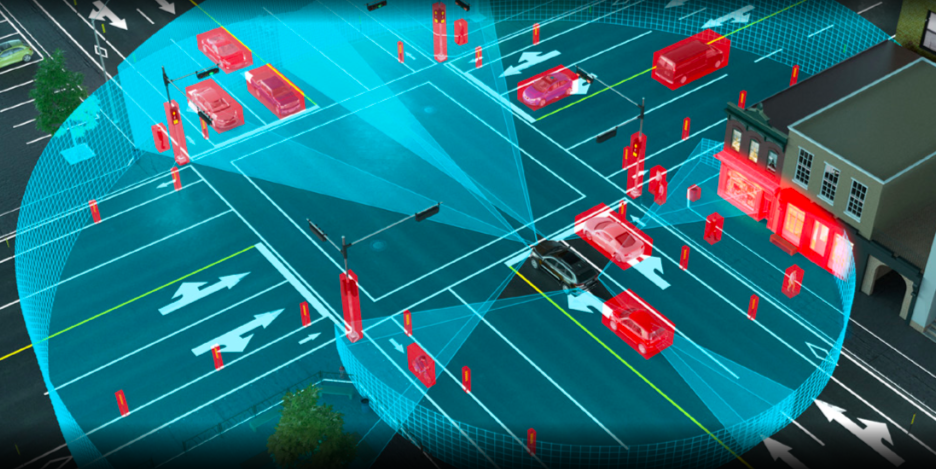
\includegraphics [width=0.7 \textwidth]{imgs/chapter2/lidarcar.png}}
\caption[Example of \ac{LiDAR} technology being used for road perception]{Example of \ac{LiDAR} technology being used for road perception \cite{lidarcar}}
\label{fig:lidarcar}
\end{figure}

One application example of this is the work done by Dominguez et al \cite{lidarperception}  where a perception system for ground vehicles was implemented using segmentation, clustering and tracking techniques.  However, it was noted by the authors that it was hard to distinguish between closely separated obstacles adding that a movement detection algorithm should be implemented to solve this problem. 


Catapamga and Ramos \cite{car2dlidar} proposed  a low cost solution for object detection, classification and ranging by the use of an inexpensive 2D pulsed light \ac{LiDAR}. The system was able to provide reliable detection of 1 meter wide obstacles at distances less than 10 meters.


However there are some concerns about this type of technology. The CEO of Tesla, Elon Musk, has been very critical of it. Recently, at Tesla’s first Autonomy Day event,  he said \textit{"Anyone relying on \ac{LiDAR} is doomed. Doomed!"} \cite{elon}. He believes that cameras, \ac{radar} and ultrasonic sensors are the future for car perception systems. 
\subsubsection{Robotics}
\ac{LiDAR} is also one of the major sensory components for robotics. Various robots rely on it for autonomous navigation. Fig. \ref{fig:robotslidar} shows an example of two robots (ROSbot and Knightscope) that use this type of sensors for perception.
\begin{figure}[ht] 
    \begin{minipage}[b]{.49\linewidth}
        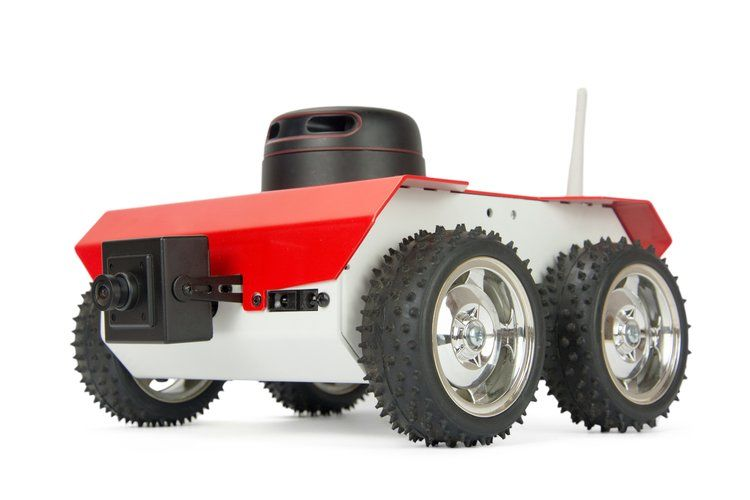
\includegraphics[height=5cm,width=\linewidth]{imgs/chapter2/robot1.jpg}
        \subcaption{ROSbot - Autonomous Robot with Laser scanner RPLiDAR A2 \cite{robot1}}
    \end{minipage}
    \begin{minipage}[b]{.49\linewidth}
        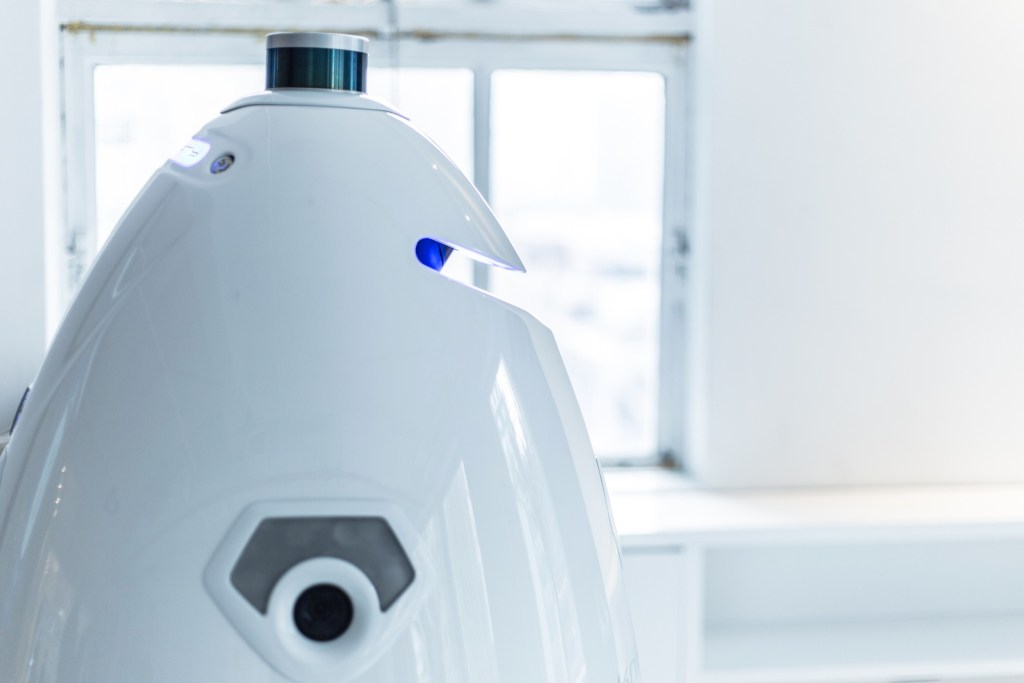
\includegraphics[height=5cm,width=\linewidth]{imgs/chapter2/robot2.jpg}
        \subcaption{Knightscope autonomous security robot with a Velodyne \ac{LiDAR} Puck \cite{robot2}}
    \end{minipage}
    \caption{Example of two robots equipped with \ac{LiDAR}}
    \label{fig:robotslidar}
\end{figure}


In one of the most popular works with robotic navigation called \textit{"The Office marathon"}  \cite{marder2010office},  the PR2 robot was able to navigate autonomously for 26.2 miles in an office like environment. During the task, the robot was able to avoid  shelves, tables, chairs and people as well as go
through narrow spaces. The sensor device used in this case was the Hokuyo UTM-30LX Scanning Laser Rangefinder and the navigation system developed is now known as the \ac{ROS} navigation stack. However it was noted that the robot had difficulty detecting low height and long width obstacles.


In a more recent case study \cite{lidar2019ros}, two different systems are proposed for the implementation of an autonomous  mobile robot, both using a 2D \ac{LiDAR} sensor under \ac{ROS}. Various trials in an indoor environment were conducted with both of them. It was concluded that both performed reasonably well but had some difficulty detecting objects with lower or higher height from the sensor, objects that are transparent, or even dark obstacles with high absorption of light waves.  

%%ADD ROBOT INDOOR NAVIGATION
\subsection{Operating Principle}
The way \ac{LiDAR} technology works is straightforward, emit a laser beam and wait for it to bounce back. Based on the propriety of the reflected signal it can determine the distance of the obstacle it hits. By constantly spinning the mirrors at different angles (scanning) it gets angle and depth information about the environment  by a  set of points or in other words a point cloud. There are two main different operating principles to do this, \textbf{Time of Flight} and \textbf{Phase Based}, which are described bellow.
\subsubsection{Time of Flight}
 In this approach a pulse of light is transmitted and,  when it is done, an internal clock is started. The reflected pulse is captured by a photodetector which triggers the clock to stop. Being $\tau$ the time taken by the reflected signal to  comeback and assuming it traveled at approximately the speed of light ($c$) then the distance to the object $d$ is given by:
\begin{equation}
    d=\frac{\tau c}{2}
\end{equation}
This method produces very accurate results for a long range but requires high precision clocks. However, greater  range capability leads to slower update rates since it has to wait more time for the pulse to comeback.
It is typically not used for robotics since this type of systems has very high cost ranging from a few thousand dollars to upwards hundreds of thousands of dollars \cite{cost}.
\subsubsection{Phase Based}
A more affordable approach  is based on modulating the intensity of the laser at a specific frequency. Figure \ref{fig:cwlidar1} showcases the resulting sinusoidal wave that is sent and the respective returned signal. 
\begin{figure}[ht!] 
\centerline{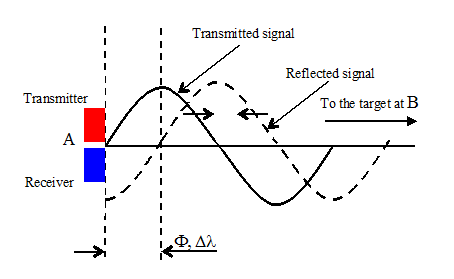
\includegraphics [width=0.7 \textwidth]{imgs/chapter2/cwlidar1.png}}
\caption[Phase based method for measuring range]{Phase based method for measuring range \cite{cwlidar}}
\label{fig:cwlidar1}
\end{figure}

Being $\Phi$ the phase difference between the transmitted signal and the reflective signal, and $\lambda_m$ the wavelength of the sinusoid then the distance of the object is given by:
\begin{equation}
    d=\frac{\Phi \lambda_m}{4 \pi}
\end{equation}
This means that the maximum unambiguous distance that can be measured is  $\frac{\lambda_m}{2}$, and its range resolution depends upon the resolution of the phase difference measurement as well as the wavelength used. Almost all robots use this type of \ac{LiDAR} since it is usually cheaper. 
%and has a faster update rate.
%difficult to generate continuous wave of high energy

\subsection{Limitations}
\ac{LiDAR} technology has some problems associated with it:
\begin{itemize}
\item{Even the most cheap devices have relative high operation costs that limit their use for small applications.}  
\item{Limited maximum detection range compared to radar technology.}  
\item{Sensors are usually bulky and fragile when compared to radar boards used in this project.} 
\item{Direct exposure to sunlight may negatively impact the sensor maximum range and accuracy or even prevent it from functioning properly.} 
\item{Slow measurement rate due to large dataset processing.} 
\item {If it is a 2D-\ac{LiDAR} it only senses in a horizontal plan}
\end{itemize}
The last item on the list proves to be a significant problem because the sensor cannot detect objects that are above or bellow the height of the sensor (Fig. \ref{fig:2dlidar}). The inability of detecting this type of objects may be crucial for the success rate of the robot being able of doing a certain navigation task safely.
\begin{figure}[ht]
    \centering
    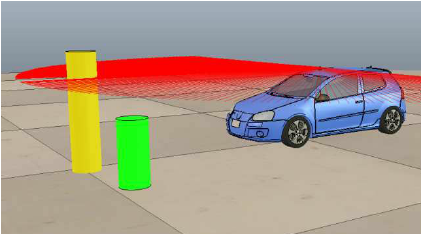
\includegraphics[scale=0.7]{imgs/chapter2/lidar2d.png}
    \caption[2D \ac{LiDAR} only detecting objects in one plane ]{2D \ac{LiDAR} only detects objects in one plane (this plane is usually parallel to the ground (taken from \cite{yalcin2013approaches})}
    \label{fig:2dlidar}
\end{figure}


\section{MIMO Linear FMCW Radar}
The use of \ac{radar} technology has been around since the 19th century when it was first discovered that radio waves reflected off metallic surfaces, but serious development of this type systems only truly began in the 1930's for military applications \cite{radarhistory}. This include the range and angle detection of ship and aircraft engines by measuring incoming signal fluctuations off an oscilloscope. 

Nowadays there are various configuration types of radar systems  \cite{typesradar}, each one providing different types of applications. This usually include air traffic control, remote sensing, ground traffic control, space, etc.  However we will focus on a specific configuration called \ac{MIMO} linear (sawtooth)  \ac{FMCW} radars which are  able to measure distance, velocity and also angular information. 

\subsection{Applications}


  \subsubsection{Pedestrian detection}  
 In \cite{heuel2010pedestrian} three systems are implemented, the first one using a single radar measurement, the second using multiple, and the final one with additional tracking algorithms. Each system had the objective of distinguishing between people walking, vehicles and other objects. In the end it was concluded that that \ac{FMCW} \ac{radar} can be used for classification of inroad objects with relatively good accuracy in all systems.
  
   Another case study is presented in \cite{knudde2017indoor} where by pre-processing the raw radar data and then using  data processing pipeline, the system proposed was able to detect and track people in indoor environments using a 77 GHz \ac{MIMO} \ac{FMCW} radar.
   
 \subsubsection{Localization of Land Vehicles}  
  Vehicle localization is often done using \ac{GNSS} accompanied by \ac{RISS}. But is often the case in which \ac{GNSS} signal can not be received correctly. This is often due the land vehicle being in an indoor environment or high rise building blocking the signal. In \cite{abosekeen2018utilizing} it is proposed a radar based \ac{RISS} that not only seeks odometer information but also radar readings. This proved to make the localization system of the vehicle more robust.
  
\subsubsection{Monitoring of human vital signs}  
Monitoring vital signs of a patient such as the breathing rate or hearth rate may be critical in some situations.
In \cite{alizadeh2019remote} a system for detecting this type of signals using  \ac{FMCW} \ac{radar} is proposed. By doing a phase analysis of the \ac{radar} signal it was concluded that the proposed system measurement was in tune with a reference ground truth signal. It was also concluded that by increasing the \ac{SNR} of \ac{radar} it could estimate the heartbeat (\ac{ECG}) waveform of multiple targets.

\subsection{Operating principle}
The \ac{MIMO} \ac{FMCW}  radar can retrieve range, velocity and angle of multiple targets. The following sections will explain how to calculate each one of these components.


An \ac{FMCW} radar transmits a signal called a “chirp”. A chirp is an electromagnetic sinusoid whose frequency  increases linearly with time. A chirp is characterized by a start frequency (fc), bandwidth (B) and duration (Tc). The slope (S) of the chirp is the rate at which the frequency of the chirp increases and is given by:
\begin{equation}
    S=\frac{B}{T_c}
\end{equation}
%% put A t and f t plot
Figure \ref{fig:At} shows the plot of the amplitude in function of time for the described chirp. It shows that the frequency of the sinusoid is increasing with time. Another way of illustrating the chirp is by its frequency plot (Fig. \ref{fig:Ft}). The latter version is often preferred because it is simpler and more intuitive.

\begin{figure}[ht] 
    \begin{minipage}[b]{.49\linewidth}
        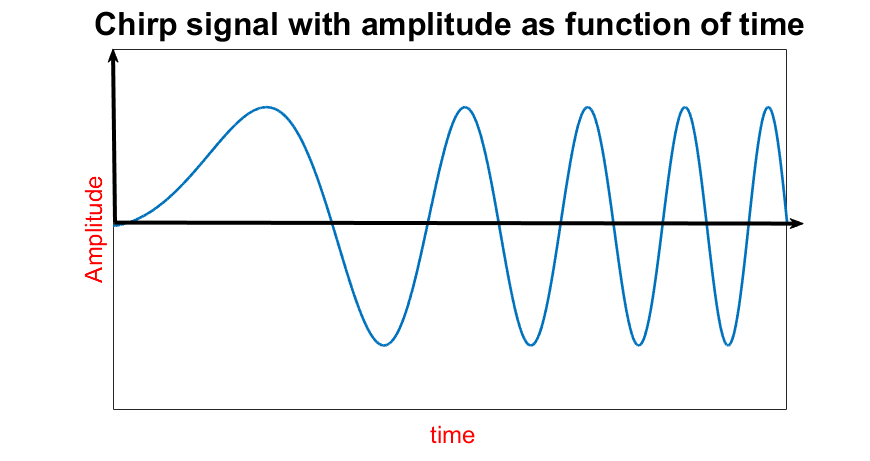
\includegraphics[height=5cm,width=\linewidth]{imgs/chapter2/chirpAt.png}
        \subcaption{Representation of the chirp, with amplitude as function of time}
        \label{fig:At}
    \end{minipage}
    \begin{minipage}[b]{.49\linewidth}
        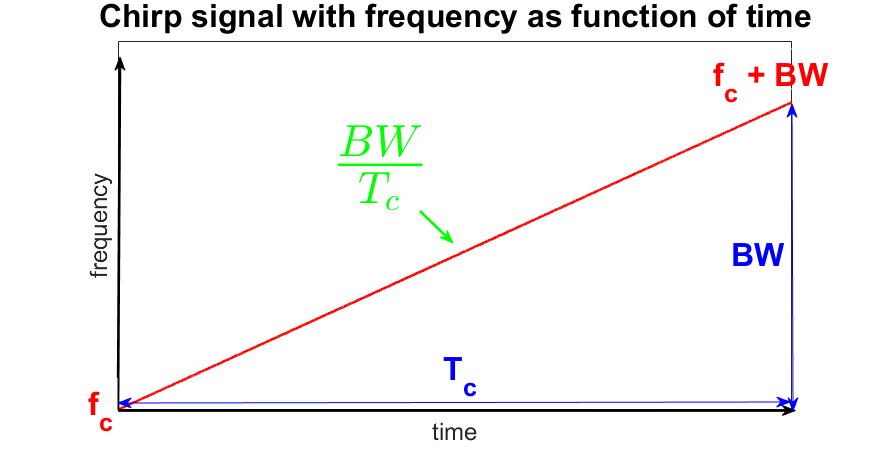
\includegraphics[height=5cm,width=\linewidth]{imgs/chapter2/chirpFt.png}
        \subcaption{Representation of the chirp, with frequency as function of time}
        \label{fig:Ft}
    \end{minipage}
    \caption{Representation of a chirp}
    \label{fig:chirp}
\end{figure}

%%PUT SOME TEXT


Object detection follows these steps:
\begin{enumerate}
    \item The chirp is transmitted by the TX antenna
    \item The chirp is reflected off an object and the reflected chirp is received at the RX antenna
    \item The RX signal and TX signal are ‘mixed’ and the resulting signal is called an ‘\ac{IF} signal’
\end{enumerate}
Figure \ref{fig:if} shows how the IF signal is generated through both the RX and TX signals for one target detection.
\begin{figure}[ht] 
\centerline{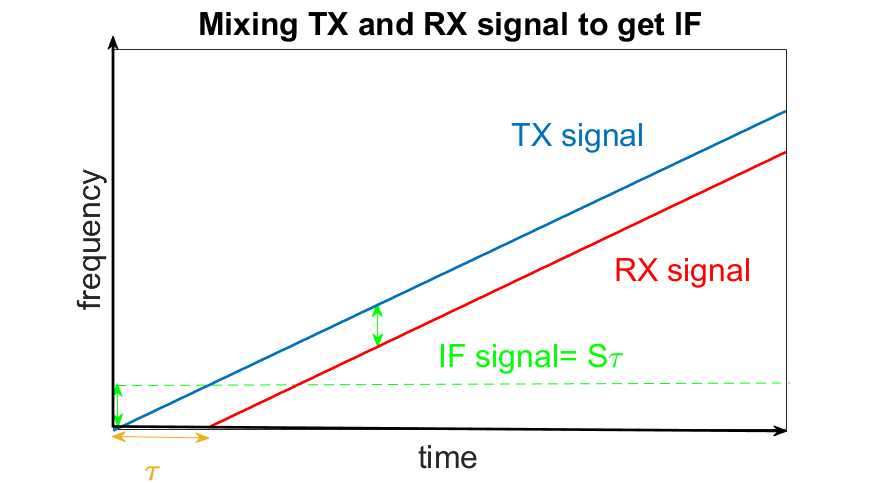
\includegraphics [width=0.8 \textwidth]{imgs/chapter2/IFsignal.png}}
\caption{IF signal creation to retrieve range information of the target}
\label{fig:if}
\end{figure}

%%PUT IMAGE
%%%When the transmitted chirp encounters an object it will reflect back to the radar and will be captured by the RX antenna.
\subsubsection{Range Detection}
The RX signal is a sum of delayed versions of the TX signal. This means that the resulting \ac{IF} signal will be a combination of sinusoids, each one corresponding to the reflection on an object. For object $i$ the corresponding frequency $f_i$ is given by:
\begin{equation}
    f_i=S\tau_i
\end{equation}
where $\tau_i$ is the round trip delay of the wave and is given by:
\begin{equation}
    \tau_i=\frac{2d_i}{c}
\end{equation}
where $d_i$ corresponds to the distance of the object to the radar and $c$ is the speed of light.
%% PUT image
Putting this together the distance to the object $i$ is given by:
\begin{equation}
    d_i=\frac{f_ic}{2S}
    \label{eq:1}
\end{equation}


To determine the range of all objects detected, we need to find the according frequency components in the \ac{IF} signal. To do this the analog signal is first sent to an \ac{ADC} and with the resulting digital output the \ac{FFT} is computed by a \ac{DSP}. Each peak in the \ac{FFT} that meets a certain \ac{SNR} threshold corresponds to a different range detection. 
 
 However since the \ac{ADC} has a limited sampling rate, the valid range of frequencies in the \ac{FFT} is also limited, this meaning there is a maximum amount of ranges the radar can detect.
The range resolution is also finite since the \ac{FFT} has a limited amount of samples. In short, the higher the bandwidth of the chirp the better resolution we get.


\subsubsection{Velocity Detection}
This type of radar also provides an estimate on the radial velocity for each detected range. To do this more than one chirp is needed. A set of N chirps is called a frame. The radar constantly sends these frames, each one corresponding to an observation. Since the time between frames is low the corresponding range (or first) \ac{FFT}s will have  identically located peaks (the same obstacle is in the same range for all chirps in a frame) . However this set of peaks have different phases between each other. By calculating a second \ac{FFT} (Doppler-FFT) of this vector of phases we can extrapolate a set of relative radial velocities  for each range detection. Radial velocity information is given by:
\begin{equation}
    v_i=\frac{\lambda \omega_i}{4 \pi T_c}
    \label{eq:2}
\end{equation}
where $\lambda$ is the wavelength of the chirp, $\omega_i$ is the phase difference between chirps for the respective objects in the Doppler FFT and $T_c$ is the time required to send a single chirp.
In the end we get a matrix that relates radial velocity and range. 
Figure \ref{fig:matrix} illustrates this process.
\begin{figure}[ht] 
\centerline{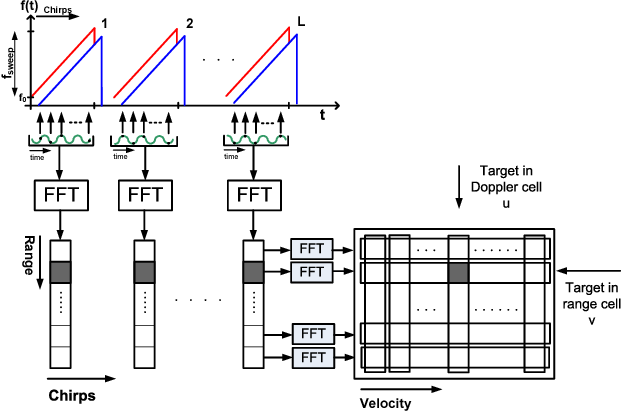
\includegraphics [width=0.7 \textwidth]{imgs/chapter2/dopplerFFT2.png}}
\caption[2D FFT for retrieving velocity information]{At the same range peaks the sinusoid has different phases, by calculating the 2D FFT (or doppler FFT) the radial velocity information can be retrieved (taken form \cite{schroeder2010x})}
\label{fig:matrix}
\end{figure}

\subsubsection{Angle Detection}
Finally, to determine the angle for each target more than one receiver antenna is needed. This is where the \ac{MIMO} configuration comes in. Figure \ref{fig:angle} shows that for the same target the distances to the two antennas is different.  This difference makes it so for the same peak in the range \ac{FFT} and doppler \ac{FFT} the phase of the received \ac{IF} signal is different in the two antennas. If we know this phase difference we can retrieve angle of arrival of the target. 
\begin{figure}[ht!] 
\centerline{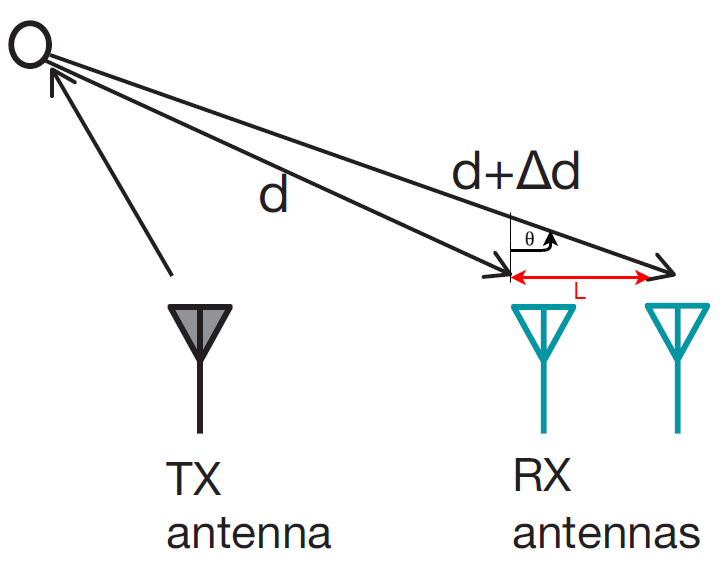
\includegraphics [width=0.7 \textwidth]{imgs/chapter2/angle2.png}}
\caption[Angle of arrival estimation using more than one antenna]{More than one antenna is required to estimate the angle of arrival (adapted form \cite{iovescu2017fundamentals})}
\label{fig:angle}
\end{figure}
The phase difference $\Delta \phi$ is given by:
\begin{equation}
    \Delta \phi=\frac{2 \pi \Delta d}{\lambda}
\end{equation}
By basic geometry we know that $\Delta d =L sin(\theta)$, where $L$ is the distance between the antennas and $\theta$ is the angle of arrival. 

\begin{equation}
    \Delta \phi=\frac{2 \pi L sin(\theta)}{\lambda}
\end{equation}
Then the angle of arrival is finallygiven by:
\begin{equation}
    \theta = sin^{-1}(\frac{\lambda \Delta \phi}{2 \pi L})
\end{equation}
The above equation makes it possible to estimate the angle of arrival. But since $\phi$ has a non linear dependency of $\sin(\theta)$ then the angle of arrival accuracy depends on the angle of arrival. The closer it is to 0º the more accurate is the result.

 
\subsection{Limitations}
\ac{FMCW} {radar} technology has some problems associated with it, some of them being:
\begin{itemize}
\item{Limited range and angular resolution when compared to \ac{LiDAR} which make difficulty to distinguish between two close targets}  
\item{Low pointcloud density}  
\item{Radar cannot provide the exact geometry of an object because of the longer wavelength}  
\item{Can have intermodulation products that result in ghost objects} 
\end{itemize}





\section{Ultrasonic Sensors}
One of the various ways  of  sensing the range of an obstacle, is by using ultrasonic sensors. Using sound waves, an ultrasonic sensor is able to measure range. 
These type of sensors have high reliability and outstanding versatility and can be used for wide variety of applications. 

\subsection{Applications}
\subsubsection{Robotics}
One examples of robotic applications is the work done by Byoung-hoon Kim \cite{kim2006improved} where by using a multi modulation processing of the ultrasonic sensors the proposed system was able to estimate the 3D coordinates of a moving object while being robust for noisy environments.
\subsubsection{Ground Vehicles}
Ultrasonic sensors is also widely used for ground vehicles. On the work  proposed by Enas Odat \cite{pir}, a traffic sensing system is constructed using \ac{PIR} sensors and ultrasonic range finders. It was able to calculate  vehicle detection, speed estimation, and vehicle type classification. However the variability of the sensors readings, thermal noise and environmental conditions may produce unwanted reading errors.
\subsubsection{Medicine}
Ultrasonic sensors are also used in medicine. For example in the work done by Ibrahim AlMohimeed et al \cite{med}, a wearable and flexible ultrasonic sensor was developed for monitoring of skeletal muscle contraction. The tissue thickness variations were successfully measured in accordance with the muscle contraction performed. 
\subsection{Operating Principle}
To retrieve range information about the environment the ultrasonic sensors work similarly as the  Time of flight \ac{LiDAR}. But instead of light waves the sensor uses sound waves. A transducer sends and receives ultrasonic pulses that relay back information about an object’s proximity.  

\begin{figure}[ht] 
\centerline{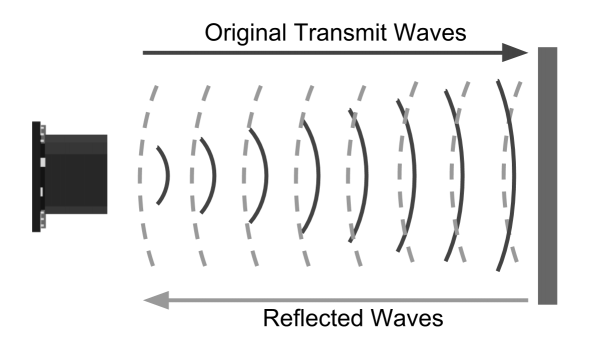
\includegraphics [width=0.8 \textwidth]{imgs/chapter2/us.png}}
\caption[Ultrasonic wave operating principle]{Ultrasonic wave operating principle (taken form \cite{burnett2019})}
\label{fig:us}
\end{figure}

\section{Cameras}
Besides the previous highlighted sensors, cameras can be used to determine the distance of obstacles. There are three image based object distance measurement techniques, (1) using two cameras i.e stereovision, (2) using a single camera and (3) time-of-flight camera \cite{cam}.
The first method is highly accurate but is costly when compared to the monovision and it is not accurate for high distances. In the time of flight technique the distance is obtained using the time it took for the light to be reflected back. This method is a simple way to retrieve range from obstacles and it is also very fast that can reach up to 160 frames per second. It is also efficient having lower computation needs when compared to stereovision. However this technique comes with the problems of background lighting, interference from other time of flight cameras and multiple reflections. 
%\subsection{Applications}
%\subsubsection{Ground Vehicles}
%The use of range cameras is widely used for ground vehicle applications. One example of this is by Canesta \cite{hsu2006performance}, where  occupant sensing and backup obstacle warning was achieved using a ranging camera.

%Another example is the work of Elkhalili et al \cite{eka}, where, by the use of these type of sensors enabled the detection of objects with a resolution of 2.2cm for a single pulse in the range up to 20m.

%\subsubsection{Robotics}
%Using this technology mobile robots can build up a map of their surroundings very quickly, enabling them to avoid obstacles or follow a leading person. As the distance calculation is simple, only little computational power is used.

%\subsection{Operating principle}
%As said before there are multiple ways in which a camera can retrieve range information. The first one is by stereovision (using two cameras). This takes into account camera calibration and the disparity map is computed that retrieves the distance of obstacles. The second way is by time of flight range cameras that work by the principle that the received signal proprieties to determine the range of obstacles.
\section{FMCW radar Simulation}
Now that we know the operating principle of the \ac{FMCW} \ac{radar} we can use the concepts for simulation purposes. In this section we explore how we can simulate in MATLAB range and velocity detection using the pre established concepts. 
\subsection{Simulating range detection}
In this section we try to simulate in MATLAB the process of retrieving the range from different targets using the \ac{FMCW} \ac{radar} operating principle. The code used to generate the simulated graphs is shown in the appendix A. Table \ref{tab:table1} shows the paramaters used for the radar and the vector of distances of the supposed objects to be retrieved, where $T_c$ is the time of chirp and $F_s$ is the sampling frequency of the \ac{ADC}.
\begin{table}[ht!]
  \begin{center}
    \caption{Parameters used for simulation for range estimation.}
    \label{tab:table1}
    \begin{tabular}{l|c} % <-- Alignments: 1st column left, 2nd middle and 3rd right, with vertical lines in between
      \textbf{Paramater} & \textbf{Value } \\
      \hline
      $f_c$ & 77 GHz \\
      Bandwidth & 4 GHz \\
      $T_c$ & 40us \\
      $F_s$ & 8 MHz \\
      Object distance & [0.2345 0.0469 1.1 3.0 5 5.3]  m
    \end{tabular}
  \end{center}
\end{table}
 Figure \ref{fig:if2} shows the TX signal in blue and RX signal as the other colors in a plot of time vs frequency.
 \begin{figure}[h] 
\centerline{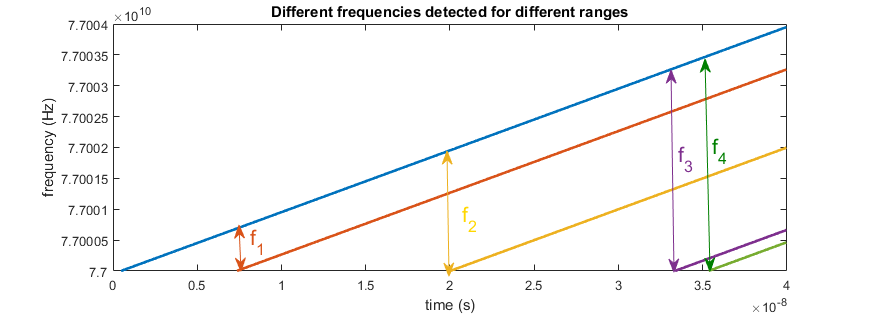
\includegraphics [width=1.0 \textwidth]{imgs/chapter2/SimFrequencies.png}}
\caption[Demonstration of the TX signal in blue and RX signal in other colours]{TX signal in blue and RX signal in other colours, each strip corresponds to a different range detection}
\label{fig:if2}
\end{figure}
%What is it
Mixing both signals and passing the resulting \ac{IF} signal by a low pass filter we then compute the \ac{FFT} of the \ac{IF} signal. Fig \ref{fig:fft} shows the result. By using equation \ref{eq:1} we can retrieve the distance vs power of the signal plot (Fig. \ref{fig:fft2}). 
\begin{figure}[ht] 
    \begin{minipage}[b]{.49\linewidth}
        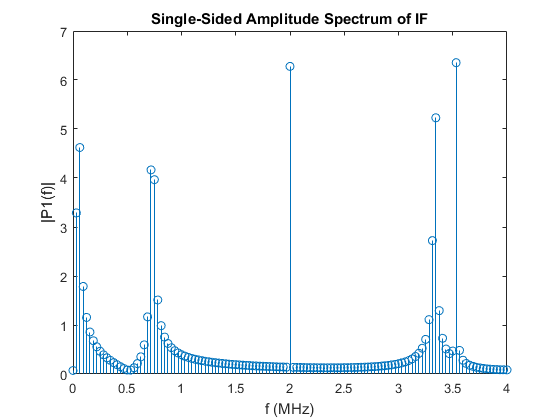
\includegraphics[height=5cm,width=\linewidth]{imgs/chapter2/FFT.png}
        \subcaption{FFT of IF signal}
        \label{fig:fft}
    \end{minipage}
    \begin{minipage}[b]{.49\linewidth}
        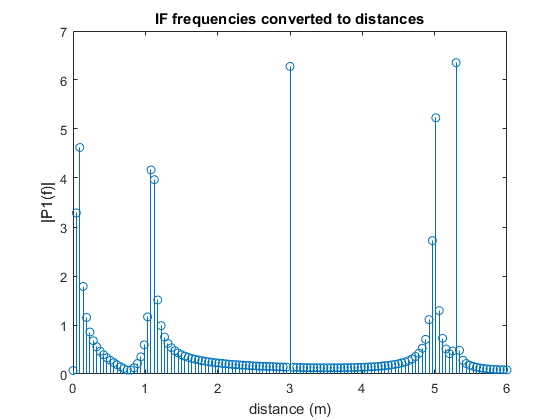
\includegraphics[height=5cm,width=\linewidth]{imgs/chapter2/distance.png}
        \subcaption{Frequencies converted to distances plot}
        \label{fig:fft2}
    \end{minipage}
    \caption{Range detection using \ac{FMCW} \ac{radar}}
    \label{fig:distancedetermination}
\end{figure}
As we can see the power of the signal is stronger in the distances that were chosen a priori. To extract them we must choose a certain threshold of \ac{SNR}. Note that the sampling frequency limits the maximum distance of detection.

\subsection{Simulating velocity detection}
In this section we try to simulate in MATLAB the process of retrieving the velocity from different targets using the \ac{FMCW} \ac{radar} operating principle. The code used to generate the simulated graphs is shown in the appendix B. Table \ref{tab:table2} shows the parameters used for the radar and the velocity and range of the supposed object to be retrieved, where $N_c$ is the number of chirps used. 
\begin{table}[ht]
  \begin{center}
    \caption{Parameters used for simulation of velocity estimation}
    \label{tab:table2}
    \begin{tabular}{l|c} % <-- Alignments: 1st column left, 2nd middle and 3rd right, with vertical lines in between
      \textbf{Paramater} & \textbf{Value } \\
      \hline
      $f_c$ & 77 GHz \\
      Bandwidth & 4 GHz \\
      $T_c$ & 40us \\
      $F_s$ & 8 MHz \\
      $N_c$ & 64 \\
      Object distance & 5  m \\
      Radial velocity & 7  m/s
    \end{tabular}
  \end{center}
\end{table}

By computing the FFT of the $N_c$ phase differences we get the 2-D doppler \ac{FFT}  for the object at 5 m.  Fig \ref{fig:fft3} shows the resulting  2D-Doppler FFT that displays which phases are stronger. By using equation \ref{eq:2} we can retrieve the velocity vs power of the signal plot (Fig. \ref{fig:fft4}). 
\begin{figure}[ht] 
    \begin{minipage}[b]{.49\linewidth}
        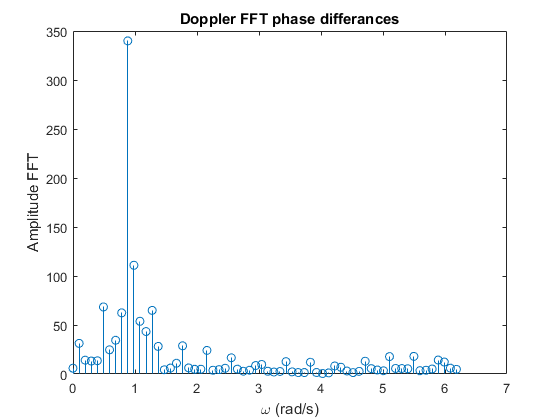
\includegraphics[height=5cm,width=\linewidth]{imgs/chapter2/fft3.png}
        \subcaption{FFT of IF signal}
        \label{fig:fft3}
    \end{minipage}
    \begin{minipage}[b]{.49\linewidth}
        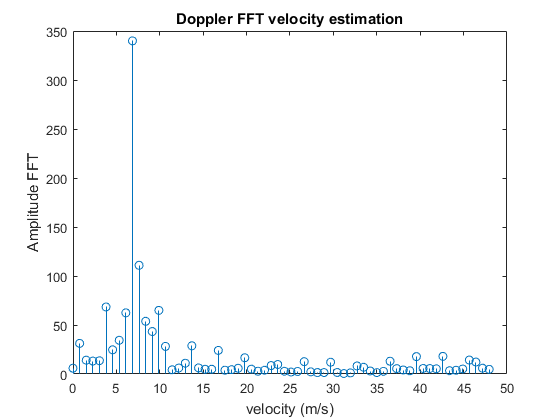
\includegraphics[height=5cm,width=\linewidth]{imgs/chapter2/fft4.png}
        \subcaption{Phase differences converted to velocity plot}
        \label{fig:fft4}
    \end{minipage}
    \caption{Velocity detection using \ac{FMCW} \ac{radar}}
    \label{fig:velocitydetermination}
\end{figure}
As we can see there is a peak near the $7 m/s$ velocity that means this parameters can be used to compute the radial velocity of the target with fairly good precision. 




\section{Summary}
In this chapter we overviewed various types of proximity sensor technologies, . First we discussed on what contexts this sensors are used for and what current work is being done with them. Then we explain the operating principle of each one of them to retrieve information from the environment as well as simulating the range and velocity estimation provided by the radar.  Finally we show what limitations each sensor has.
%GIVE OVERVIEW OF THE CURRENT SENSORS LEADING INDOOR NAVIGATION.





